\section{Metodologia}
	
	O processo metodológico escolhido para desenvolvimento do R2-PI2 é baseado em uma metodologia ágil, mais especificamente, no \textit{Scrum}. Dessa forma, o processo como um todo será dividido \textit{releases}, contemplando \textit{sprints} de 2 semanas, em média. Antes de definirmos o processo de maneira específica, é necessário apresentar uma visão alto nível do projeto inteiro, destacando os pontos de controle e deixando claras as atividades críticas para o sucesso do projeto.

	Com este objetivo, o processo apresentado na Figura \ref{img:processo_geral} foi modelado, utilizando a ferramenta \textit{Bizagi Modeler}\footnote{http://www.bizagi.com/pt/}.

	\begin{figure}[H]
		\centering
		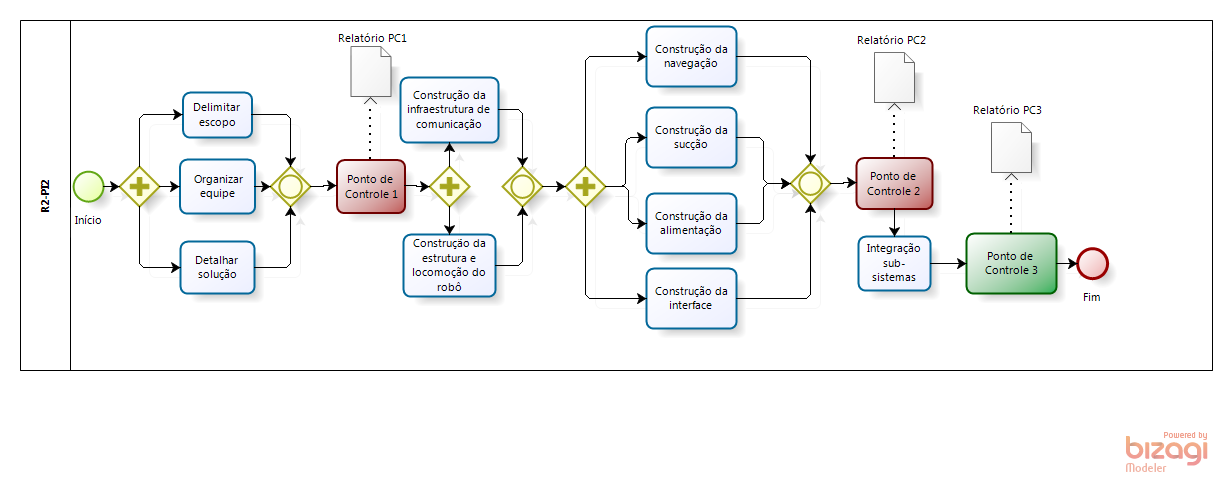
\includegraphics[scale=0.55]{figuras/processo_geral.png}
		\caption{Processo geral de desenvolvimento da solução.}
		\label{img:processo_geral}
	\end{figure}

	As atividades presentes no processo estão descritas abaixo.

	\begin{itemize}
		\item \textbf{Delimitar escopo}:

			Etapa de levantamento dos requisitos, onde é definido tudo que está dentro do projeto, que será implementado, e tudo que está fora, ou seja, que não será implementado.

		\item \textbf{Organizar equipe}:

			Etapa que busca definir uma política de comunicação da equipe, discute e define com todos os integrantes a metodologia e a rotina de trabalho que serão seguidas e define papéis e/ou responsabilidades.

		\item \textbf{Detalhar solução}:

			Etapa onde são divididos subsistemas que integrados solucionarão o problema inicial. Cada equipe responsável por determinado subsistema deverá identificar soluções viáveis, apresentar a solução mais adequada e detalhar a mesma. Com a união do detalhamento de todos os subsistemas, obtem-se o detalhamento geral do sistema.

		\item \textbf{Ponto de Controle 1}:

			Primeiro ponto de controle do projeto, etapa onde é entregue o relatório 1, contemplando toda a organização da equipe e da metodologia de trabalho, o escopo bem definido, a solução planejada (de forma detalhada) e o plano de riscos do projeto.

		\item \textbf{Construção da infraestrutura de comunicação}:

			Esta etapa envolve uma das duas atividades consideradas críticas durante este projeto. Esta característica se dá pois o seu resultado sustentará o desenvolvimento das soluções seguintes, assim como a próxima etapa a ser apresentada. Nesta etapa será implementada a rede de comunicação entre a \textit{raspberry} e o \textit{arduino}, possibilitando o envio e recebimento de informações de ambos os lados.

		\item \textbf{Construção da estrutura e locomoção do robô}:

			Durante esta etapa, que também é uma etapa crítica do projeto, está envolvida a construção da estrutura do robô, ou seja, a estrutura que sustentará todos os equipamentos presentes no robô, e o sistema de locomoção do mesmo. Possuindo o sistema de locomoção e a estrutura prontos, o robô já será capaz de responder a sinais vindos da \textit{raspberry}, de acordo com a etapa anterior.

		\item \textbf{Construção da navegação}:

			Esta etapa se refere a construção do algoritmo de navegação utilizado na solução, ou seja, se preocupa com o controle do robô em relação a sua trajetória de locomoção pelo cômodo.

		\item \textbf{Construção da sucção}:

			Esta etapa envolve a construçao de todo o sistema de sucção, possibilitando a limpeza do cômodo.

		\item \textbf{Construção da alimentação}:

			Esta etapa envolve a implementação de toda a solução referente a alimentação energética do sistema, tanto em relação a bateria quando à recarga da mesma.

		\item \textbf{Construção da interface}:

			Esta etapa se preocupa com a iteração Humano-Computador envolvida nesta solução. como resultado desta atividade, espera-se uma interface amigável e de fácil aprendizado, seja no modo site ou físico.

		\item \textbf{Ponto de Controle 2}:

			Segundo ponto de controle do projeto, referente a entrega dos subsistemas prontos, funcionando separadamente. Envolve a entrega do relatório 2, constando todo o processo de desenvolvimento e a solução utilizada até o momento.

		\item \textbf{Integração subsistemas}:

			Esta etapa tem como objetivo integrar todos os subsistemas já construídos, gerando a solução com funcionamento geral.

		\item \textbf{Ponto de Controle 3}:

			Entrega final do projeto, apresentação da solução final.
	\end{itemize}

	O processo apresentado acima contempla todo o caminho a ser percorrido durante o projeto R2-PI2, porém é necessário também especificar o processo metodológico utilizado pela equipe, o qual será baseado no \textit{Scrum} e é apresentado na Figura 


	\begin{figure}[H]
		\centering
		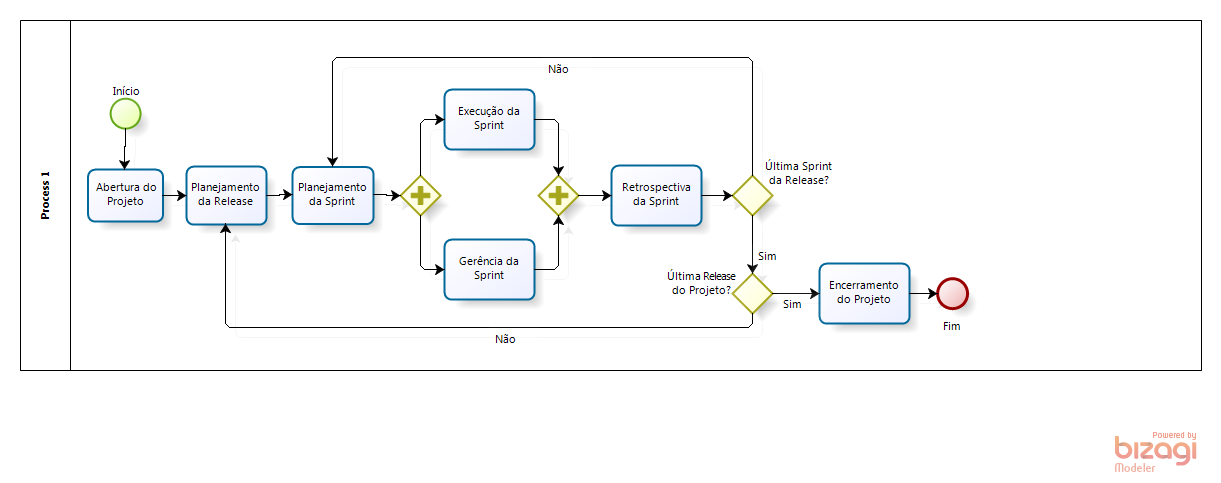
\includegraphics[scale=0.55]{figuras/processo_scrum.png}
		\caption{Processo metodológico de desenvolvimento da solução.}
		\label{img:processo_scrum}
	\end{figure}


	As atividades presentes no processo estão descritas abaixo.

	\begin{itemize}
		\item \textbf{Abertura do projeto}:

			Etapa inicial do projeto, onde são definidos o escopo do projeto, a equipe de desenvolvimento, a quantidade de releases, a divisão dos entregáveis de cada release e os rituais do scrum a serem seguidos.

		\item \textbf{Planejamento da Release}:

			Etapa onde são definidos quais são as tarefas a serem realizadas durante a release, incluindo tarefas que cumpram o objetivo da release e eventuais dívidas técnicas.

		\item \textbf{Planejamento de Sprint}:

			Etapa onde são definidas e distribuídas as tarefas da sprint para os desenvolvedores de acordo com suas capacidades e potenciais.

		\item \textbf{Execução da Sprint}:

			Etapa que dura 2 semanas, onde são desenvolvidas as tarefas definidas no planejamento da sprint.

		\item \textbf{Gerência da Sprint}:

			Paralelo a execução da sprint, a gerência da sprint é a etapa onde o scrum master ajuda os desenvolvedores a realizar suas tarefas e a garantir que as atividades processuais sejam feitas corretamente.

		\item \textbf{Retrospectiva da Sprint}:

			Etapa onde os desenvolvedores expõem para o resto da equipe os fatores positivos e negativos e pontos de melhoria para que as próximas sprints não cometam os mesmos erros e sigam com as coisas boas.

		\item \textbf{Encerramento do Projeto}:

			Nesta etapa, é realizada a formalização da entrega do produto final.

	\end{itemize}

	\subsection{Cronograma} % (fold)
	\label{sub:cronograma}
		
		O cronograma do projeto foi desenvolvido com a utilização da ferramenta \textit{Gantter}, que pode ser acessado via \href{https://www.smartapp.com/gantterforgoogledrive/index.html?fileID=0B7s5Po6PeeDMV2RhY2dWVEUtTUU#}{Google Drive}, e está visível na Figura \ref{img:cronograma}.

		\begin{figure}[H]
			\centering
			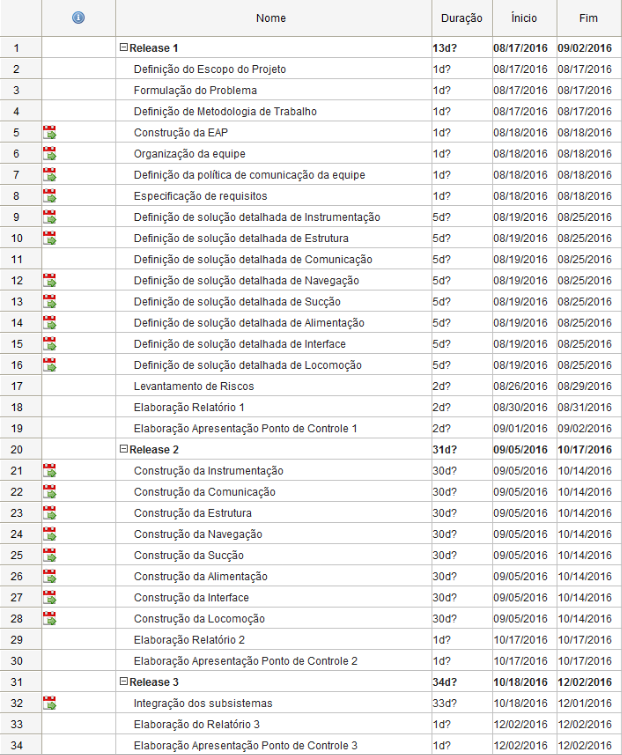
\includegraphics[scale=0.8]{figuras/cronograma.png}
			\caption{Cronograma do projeto}
			\label{img:cronograma}
		\end{figure}
	% subsection cronograma (end)
